\documentclass{beamer}

% --- Presentation Theme ---
\usetheme{default} % A clean, professional theme with navigation bars.
%\usecolortheme{beaver} % A pleasant, high-contrast color scheme.
\setbeamercolor{block title}{bg=blue!20!white,fg=black} % Lighter block titles
\setbeamercolor{block body}{bg=blue!5!white}
\setbeamercovered{transparent} % Fades out unrevealed items.

% --- Packages ---
\usepackage[utf8]{inputenc}
\usepackage{amsmath}
\usepackage{amssymb}
\usepackage{amsfonts}
\usepackage{tikz}
\usetikzlibrary{calc, shapes.geometric}
\usepackage{braket}      % For professional quantum mechanics notation (e.g., \ket{}, \bra{})
\usepackage{siunitx}     % For consistent and well-formatted units (e.g., \SI{1.585}{bits})

% --- Custom Commands for Consistency ---
\newcommand{\Hfull}{H_{\text{full}}}
\newcommand{\Hcoll}{H_{\text{coll}}}
\newcommand{\HcaseA}{H_{\text{case A}}}
\newcommand{\HcaseB}{H_{\text{case B}}}
\newcommand{\obs}[1]{#1_{\text{obs}}} % For observed states

% --- Metadata ---
\title{Chromatic Quantum Contextuality}
\author{Karl Svozil}
\institute{Institute for Theoretical Physics, TU Wien, Vienna}
\date{IQSA2025, Tropea, Calabria (Italy) \textbullet{} 2025-06-30\\ $\;$\\
\footnotesize Gemini 2.5 Pro (final 6/27) enhanced version\\ $\;$\\
\small \url{http://tph.tuwien.ac.at/~svozil/publ/2025-IQSA-pres-Svozil.pdf}}

\begin{document}

% --- Title Page ---
\begin{frame}
    \titlepage
\end{frame}


\begin{frame}
    \frametitle{Teaser: What's wrong with these color-assignments-as measurement-outcomes? If so, could this be improved?}

    \begin{center}
            % --- FIGURE 2 (Your "Pink" Version) ---
            \resizebox{0.45\textwidth}{!}{%
                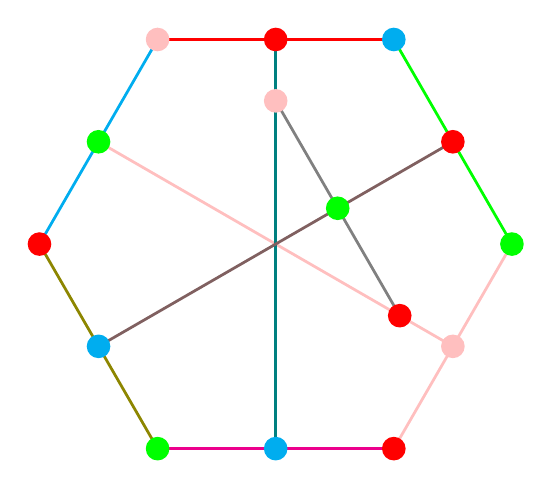
\begin{tikzpicture}
                    \tikzset{
                        every path/.style={line width=1pt},
                        c3/.style={circle, inner sep={0.05cm/8}, minimum size=6*0.05cm},
                        c2/.style={circle, inner sep={0.05cm/8}, minimum size=4*0.05cm},
                        c1/.style={circle, inner sep={0.05cm/8}, minimum size=0.8*0.05cm}
                    }
                    \def\R{30mm}
                    \path
                    ({ 180 - 0 * 360 /6}:\R)      coordinate(1)
                    ({ 180 - 30 - 0 * 360 /6}:{\R * sqrt(3)/2})      coordinate(2)
                    ({ 180 - 1 * 360 /6}:\R)   coordinate(3)
                    ({ 180 - 30 - 1 * 360 /6}:{\R * sqrt(3)/2})   coordinate(4)
                    ({ 180 - 2 * 360 /6}:\R)  coordinate(5)
                    ({ 180 - 30 - 2 * 360 /6}:{\R * sqrt(3)/2})  coordinate(6)
                    ({ 180 - 3 * 360 /6}:\R)  coordinate(7)
                    ({ 180 - 30 - 3 * 360 /6}:{\R * sqrt(3)/2})  coordinate(8)
                    ({ 180 - 4 * 360 /6}:\R)     coordinate(9)
                    ({ 180 - 30 - 4 * 360 /6}:{\R * sqrt(3)/2})     coordinate(10)
                    ({ 180 - 5 * 360 /6}:\R)     coordinate(11)
                    ({ 180 - 30 - 5 * 360 /6}:{\R * sqrt(3)/2})     coordinate(12);
                    \draw [color=cyan] (1) -- (2) -- (3);
                    \draw [color=red] (3) -- (4) -- (5);
                    \draw [color=green] (5) -- (6) -- (7);
                    \draw [color=pink] (7) -- (8) -- (9);
                    \draw [color=magenta] (9) -- (10) -- (11);
                    \draw [color=olive] (11) -- (12) -- (1);
                    \draw [color=pink] (2) -- (8)  coordinate[pos=0.85]  (15);
                    \draw [color=teal] (4) -- (10)  coordinate[pos=0.15]  (13);
                    \draw [color=pink!50!black] (6) -- (12)  coordinate[pos=0.325]  (14);
                    \draw [color=gray] (13) --(15);
                    \draw (1) coordinate[c3,fill=red ];
                    \draw (2) coordinate[c3,fill=green ];
                    \draw (3) coordinate[c3,fill=pink ];
                    \draw (4) coordinate[c3,fill=red ];
                    \draw (5) coordinate[c3,fill=cyan ];
                    \draw (6) coordinate[c3,fill=red ];
                    \draw (7) coordinate[c3,fill=green ];
                    \draw (8) coordinate[c3,fill=pink ];
                    \draw (9) coordinate[c3,fill=red ];
                    \draw (10) coordinate[c3,fill=cyan ];
                    \draw (11) coordinate[c3,fill=green ];
                    \draw (12) coordinate[c3,fill=cyan ];
                    \draw (13) coordinate[c3,fill=pink ];
                    \draw (14) coordinate[c3,fill=green ];
                    \draw (15) coordinate[c3,fill=red ];
                \end{tikzpicture}
            } % end of resizebox
    \end{center}

\end{frame}

%==================================================================
\section{Quantum Contextuality}
%==================================================================

% To be placed in the preamble of your document:
% \usepackage{hyperref}
% \hypersetup{colorlinks=true, urlcolor=blue, linkcolor=blue, citecolor=blue}

% To be placed in the preamble of your document:
% \usepackage{hyperref}
% \hypersetup{colorlinks=true, urlcolor=blue, linkcolor=blue, citecolor=blue}

% --- SLIDE 1 ---
\begin{frame}{The General Strategy I: Physical Setup}
\small
    \begin{itemize}[<+->] % Reveals items one by one
        \item We begin with a finite collection of \alert{maximal quantum observables}, also known as contexts, blocks, or subalgebras.
        \begin{itemize}[<+->] % Reveals items one by one
            \item They are (with rare exceptions such as Bell's original or CHSH configurations) chosen to be \alert{intertwining} (Gleason, 1957, \href{https://doi.org/10.1512/iumj.1957.6.56050}{doi:10.1512/iumj.1957.6.56050}) or overlapping, existing in a Hilbert space of dimension $d \ge 3$.
            \item Maximal observables have the finest spectral resolution and comprise ``all information obtainable from a quantized system at a time''
(von Neumann, 1931, Satz 8, \href{https://doi.org/10.2307/1968185}{doi:10.2307/1968185})
        \end{itemize}
       % \vspace{1.5em}
        \item This physical system is then represented by a \alert{$d$-uniform Greechie-type hypergraph}---a
graph-theoretic structure derived from the quantum model which has a Faithful Orthogonal Representation
(FOR, Lov\'asz, 1979, \href{https://doi.org/10.1109/TIT.1979.1055985}{doi:10.1109/TIT.1979.1055985})
in terms of (unit) vectors, or one-dimensional orthogonal projection operators.
By its non-degenerate spectral decomposition, every such context or block can be identified with a maximal observable.
    \end{itemize}
\end{frame}


% --- SLIDE 2 ---
\begin{frame}[shrink]{The General Strategy I (cntd): Analysis via Two-Valued States}
\small
    We analyze the hypergraph's ``classical performance'' by assigning \alert{two-valued states} (truth values $\{1, 0\}$ or $\{$true, false$\}$) to the observables.
%
    This method allows us to determine if the system exhibits:
    \begin{itemize} [<+->] % Reveals items one by one
        \item \textbf{Logical Classical Constraints:} Forced correlations like True-Implies-False (TIFS) or `Hardy-type' True-Implies-True (TITS).
        \vspace{1em}
        \item \textbf{Classical Nonseparability:} Certain observables must be assigned the same truth value in all possible states (cf. Kochen \& Specker, 1968, Separation Criterion in Theorem 0, \href{https://doi.org/10.1512/iumj.1968.17.17004}{doi:10.1512/iumj.1968.17.17004}).
        \vspace{1em}
        \item \textbf{Kochen-Specker (KS) Contextuality:} Configurations where the set of admissible two-valued states is \alert{empty},
proving a complete contradiction (by proof-by-contradiction) with classical assumptions.
    \end{itemize}
\end{frame}


% --- SLIDE 3 ---
\begin{frame}{The General Strategy I (cntd): Connection to Probability}
    \begin{itemize}[<+->] % Reveals items one by one
        \item The complete set of two-valued states can be used to construct all classical probability distributions via \alert{convex summation}.
        \item The convex hull of these states forms the \alert{classical correlation polytope}.
        \item \alert{Bell-Type Inequalities From Hull Computation:} The facets of this polytope mathematically define all
possible  Bell-type inequalities
for the system\\
{\small (Froissart, 1981, \href{https://doi.org/10.1007/BF02903286}{doi:10.1007/BF02903286}; \\
Pitowski, 1986, \href{https://doi.org/10.1063/1.527066}{doi:10.1063/1.527066}).}
\item
This remains true even for \alert{intertwining contexts/blocks}\\
{\small (KS, 2001, \href{https://doi.org/10.48550/arXiv.quant-ph/0012066}{doi:10.48550/arXiv.quant-ph/0012066}); \\
Klyachko, 2008, Can, Ali, Sinem \& Shumovsky, \href{https://doi.org/10.1103/PhysRevLett.101.020403}{doi:10.1103/PhysRevLett.101.020403}). }
    \end{itemize}
\end{frame}


% --- SLIDE 4 ---
\begin{frame}[shrink=5]{An Alternative Strategy II: Analysis via Graph Colorings}
    \begin{itemize} [<+->] % Reveals items one by one
        \item We again start with the same \alert{$d$-uniform hypergraph} representing the quantum system.
        \vspace{1.5em}
        \item Instead of truth values, we analyze the system using \alert{graph colorings}. A valid coloring assigns a ``color''
(a distinct outcome) to each observable such that all $d$ observables within any single context (hyperedge) receive different colors.
        \vspace{1.5em}
        \item This approach reveals contextual properties, such as:
        \begin{itemize}[<+->] % Reveals items one by one
            \item \textbf{Forced Correlations:} Whether certain observables must have the same or different colors in every valid coloring.
            \vspace{1em}
            \item \textbf{Generalized KS Theorem:} Contextuality is proven if the \alert{chromatic number $\chi(G)$} (the minimum number of colors needed) \alert{exceeds the dimension $d$}: $\chi(G) > d$.
 This shows it is impossible to assign $d$ distinct outcomes per context consistently.
        \end{itemize}
    \end{itemize}
\end{frame}

\begin{frame}{Postulate/Presumption of Chromatic Classicality, Aggregated Two-Valued States}
\small
Suppose a $d$-uniform hypergraph, that is, every hyperedge contains $d$ vertices (elements).
\begin{itemize} [<+->] % Reveals items one by one
        \item \textbf{Chromatic Noncontextuality:} The color (value) of intertwining observables is independent of the (hyper)edge.
        \item \textbf{Chromatic Reality:} Existence of classical distinct $d$-ary elements of physical reality for all contexts/blocks
of a $d$-uniform hypergraph.
        \item \textbf{Aggregated Two-Valued States:} Two-valued states derived from an irreversible (many-to-two)
\alert{``collapse'' or ``reduction'' or ``condensation'' of a $d$-coloring} by identifying
a single color with the value ``1'', and the remaining with the value ``0''
(Meyer, 1999, \href{https://doi.org/10.1103/PhysRevLett.83.3751}{doi:10.1103/PhysRevLett.83.3751}).
 \item Every $d$-coloring induces a canonical $d$-partitioning of all vertices (elements) of the hypergraph
(Shekarriz \& KS, 2022, \href{https://doi.org/10.1063/5.0062801}{doi:10.1063/5.0062801}).
%it represents an what is an  independent vertex cover (Shekarriz, 2025, private communication).
\end{itemize}
\end{frame}


\begin{frame}
\frametitle{Information Loss from Asymmetric Aggregation}
\small % Use smaller font for the entire frame

\textbf{Scenario:} An experiment with \textbf{n equiprobable outcomes} is aggregated into two groups: \{1 outcome\} $\to$ "1" and \{d-1 outcomes\} $\to$ "0".

\vspace{1em}

\begin{columns}[T]
    \begin{column}{0.5\textwidth}
        \begin{block}{1. Initial Information (in bits)}
            $H_{\text{initial}} = \log_2(d)$
        \end{block}

        \begin{block}{2. Aggregated Information}
            $H_{\text{final}} = H\left(\frac{1}{d}, \frac{d-1}{d}\right)$
        \end{block}

        \begin{block}{3. Information Loss (in bits)}
            The loss simplifies to:
            \begin{equation*}
                \text{Loss} = \frac{d-1}{n} \log_2(d-1)
            \end{equation*}
        \end{block}
    \end{column}

    \begin{column}{0.5\textwidth}
        \begin{block}{4. Examples (in bits)}
            \centering
            \begin{tabular}{r|cc}
                \textbf{d} & \textbf{Initial H} & \textbf{Loss} \\
                \hline
                \rule{0pt}{1.1em}%
                \textbf{2} & $1.000$ & $\mathbf{0.000}$ \\
                \rule{0pt}{1.1em}%
                \textbf{3} & $1.585$ & $\mathbf{0.667}$ \\
                \rule{0pt}{1.1em}%
                \textbf{4} & $2.000$ & $\mathbf{1.189}$ \\
            \end{tabular}
            \vspace{0.5em}

            \textit{Note: The loss for d=2 is zero because aggregation is just a one-to-one relabeling.}
        \end{block}
    \end{column}
\end{columns}

\end{frame}


% A command for a bold number, makes it stand out




\begin{frame}
\frametitle{Asymptotic Behavior: Fraction of Information Lost}
\small % Use a smaller font size to ensure everything fits

\textbf{Question:} What fraction of information is lost as the number of outcomes, \textit{d}, tends to infinity?

\begin{block}{Limit of the Loss Ratio}
The fraction of lost information is the ratio of the loss to the initial entropy:
\[
    \text{Fraction} = \frac{\text{Loss}}{H_{\text{initial}}} = \frac{\frac{d-1}{d} \log_2(d-1)}{\log_2(d)}
\]
We evaluate the limit as $d \to \infty$:
\[
    \lim_{d \to \infty} \underbrace{\left( \frac{d-1}{d} \right)}_{\to 1} \cdot \underbrace{\left( \frac{\log_2(d-1)}{\log_2(d)} \right)}_{\to 1 \text{ (by L'H\^{o}pital's Rule)}}
\]
\end{block}

\begin{alertblock}{Conclusion: A Total Information Loss}
The limit of the fraction is $1 \times 1 = \textbf{1}$.
%\vspace{0.2em}
This means that as the number of initial outcomes grows infinitely large, we lose effectively \textbf{100\%} of the initial information.
\end{alertblock}

\end{frame}





\begin{frame}{One Coloring Instance of Three-coloring in 3 Dimensions: Star-like hypergraph}
    \begin{columns}[c] % Vertically center columns
        \begin{column}{0.45\textwidth}
            \resizebox{\textwidth}{!}{
                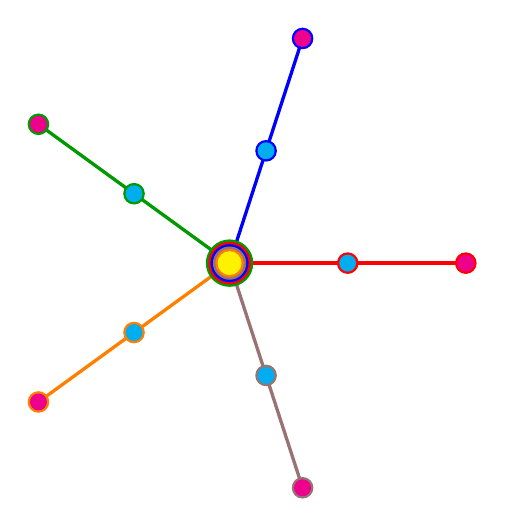
\begin{tikzpicture}
                  % --- Definitions ---
                  \def\centralRadius{0.13cm}
                  \def\centralwRadius{0.16cm}
                  \def\centralwwRadius{0.19cm}
                  \def\centralwwwRadius{0.22cm}
                  \def\centralwwwwRadius{0.25cm}
                  \def\centralwwwwwRadius{0.28cm}
                  \def\rayLength{3cm}
                  \def\smallCircleRadius{0.13cm}
                  \def\smallerCircleRadius{0.1cm}
                  \def\lineWidth{very thick}

                  % --- Rays and Outer Circles ---
                  % CORRECTED 'Green' to 'green' (lowercase) to avoid package error.
                  \foreach \angle/\rayColor in {0/red, 72/blue, 144/green!60!black, 216/orange, 288/pink!60!black} {
                    \draw[color=\rayColor, \lineWidth] (0,0) -- (\angle:\rayLength);
                    \filldraw[color=\rayColor] (\angle:{\rayLength/2}) circle (\smallCircleRadius);
                    \filldraw[color=cyan] (\angle:{\rayLength/2}) circle (\smallerCircleRadius);
                    \filldraw[color=\rayColor] (\angle:\rayLength) circle (\smallCircleRadius);
                    \filldraw[color=magenta] (\angle:\rayLength) circle (\smallerCircleRadius);
                  }
                  % --- Central Atom ---
                  \filldraw[green!60!black, \lineWidth] (0,0) circle (\centralwwwwwRadius);
                  \filldraw[red, \lineWidth] (0,0) circle (\centralwwwwRadius);
                  \filldraw[blue, \lineWidth] (0,0) circle (\centralwwwRadius);
                  \filldraw[pink!60!black, \lineWidth] (0,0) circle (\centralwwRadius);
                  \filldraw[orange, \lineWidth] (0,0) circle (\centralwRadius);
                  \filldraw[yellow, \lineWidth] (0,0) circle (\centralRadius);
                \end{tikzpicture}
            }
        \end{column}
        \begin{column}{0.55\textwidth}
            %\begin{block}{Interpretation}
            \begin{itemize}[<+->] % Reveals items one by one
                \item The center \alert{\color{yellow}yellow} atom on the intertwining element maps to value 1.
                \item All other atoms with colors \alert{\color{cyan}cyan} and \alert{\color{magenta}magenta} (subtractive primary coloring scheme) map to two respective values 2 and 3.
            \end{itemize}
            In Hilbert space, this corresponds to projecting onto respective 1D subspaces---corresponding to maximal operators with non-degenerate maximal resolution; no degeneracy there.
            %\end{block}
        \end{column}
    \end{columns}
\end{frame}

\begin{frame}{Two-Valued State in 3 Dimensions Aggregated From Coloring: Star-like hypergraph}
    \begin{columns}[c] % Vertically center columns
        \begin{column}{0.45\textwidth}
            \resizebox{\textwidth}{!}{
                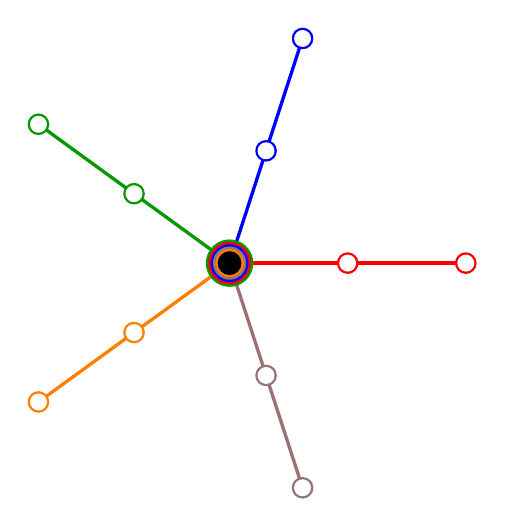
\begin{tikzpicture}
                  % --- Definitions ---
                  \def\centralRadius{0.13cm}
                  \def\centralwRadius{0.16cm}
                  \def\centralwwRadius{0.19cm}
                  \def\centralwwwRadius{0.22cm}
                  \def\centralwwwwRadius{0.25cm}
                  \def\centralwwwwwRadius{0.28cm}
                  \def\rayLength{3cm}
                  \def\smallCircleRadius{0.13cm}
                  \def\smallerCircleRadius{0.1cm}
                  \def\lineWidth{very thick}

                  % --- Rays and Outer Circles ---
                  % CORRECTED 'Green' to 'green' (lowercase) to avoid package error.
                  \foreach \angle/\rayColor in {0/red, 72/blue, 144/green!60!black, 216/orange, 288/pink!60!black} {
                    \draw[color=\rayColor, \lineWidth] (0,0) -- (\angle:\rayLength);
                    \filldraw[color=\rayColor] (\angle:{\rayLength/2}) circle (\smallCircleRadius);
                    \filldraw[color=white] (\angle:{\rayLength/2}) circle (\smallerCircleRadius);
                    \filldraw[color=\rayColor] (\angle:\rayLength) circle (\smallCircleRadius);
                    \filldraw[color=white] (\angle:\rayLength) circle (\smallerCircleRadius);
                  }
                  % --- Central Atom ---
                  \filldraw[green!60!black, \lineWidth] (0,0) circle (\centralwwwwwRadius);
                  \filldraw[red, \lineWidth] (0,0) circle (\centralwwwwRadius);
                  \filldraw[blue, \lineWidth] (0,0) circle (\centralwwwRadius);
                  \filldraw[pink!60!black, \lineWidth] (0,0) circle (\centralwwRadius);
                  \filldraw[orange, \lineWidth] (0,0) circle (\centralwRadius);
                  \filldraw[black, \lineWidth] (0,0) circle (\centralRadius);
                \end{tikzpicture}
            }
        \end{column}
        \begin{column}{0.55\textwidth}
            %\begin{block}{Interpretation}
            This (Greechie-type) hypergraph represents an aggregated system:
            \begin{itemize} [<+->] % Reveals items one by one
                \item The center atom, previously colored \alert{\color{yellow}yellow}, is now assigned the value 1, indicated by \alert{black}.
                \item All \alert{non-center} atoms, previously colored \alert{\color{cyan}cyan} or \alert{\color{magenta}magenta},
are now assigned the value $0$, indicated by \alert{white}.
            \end{itemize}
            In Hilbert space, this corresponds to projecting onto a 1D subspace vs. its orthogonal $(d-1)$D complement resulting in
a ``degeneracy of outcomes'' and a non-maximal operator with degenerate spectrum.
            %\end{block}
        \end{column}
    \end{columns}
\end{frame}







% --- Define the data for the 5 colorings (for atoms 1-10) ---
\def\coloringOneData{1,2,3,1,2,1,3,1,2,3}
\def\coloringTwoData{1,2,3,1,2,3,1,2,3,2}
\def\coloringThreeData{1,2,3,1,2,3,1,3,2,3}
\def\coloringFourData{1,2,3,2,1,2,3,1,2,3}
\def\coloringFiveData{1,2,3,2,1,3,2,1,3,2}

% --- Define the data for the 10 two-valued states (CORRECTED) ---
\def\stateOneData{1,0,0,1,0,1,0,1,0,0}
\def\stateTwoData{1,0,0,1,0,0,1,0,0,0}
\def\stateThreeData{1,0,0,0,1,0,0,1,0,0}
\def\stateFourData{0,1,0,1,0,1,0,0,1,0}
\def\stateFiveData{0,1,0,1,0,0,1,0,0,1}
\def\stateSixData{0,1,0,0,1,0,0,1,0,1}
\def\stateSevenData{0,1,0,0,1,0,0,0,1,0}
\def\stateEightData{0,0,1,0,0,1,0,1,0,1}
\def\stateNineData{0,0,1,0,0,1,0,0,1,0}
\def\stateTenData{0,0,1,0,0,0,1,0,0,1}

% --- Define the center colors ---
\colorlet{colorCode1}{yellow}
\colorlet{colorCode2}{cyan}
\colorlet{colorCode3}{magenta}
\colorlet{stateColor0}{white}
\colorlet{stateColor1}{black}

% --- Generic master command to draw one pentagon ---
% #1: The list of 10 center color codes
% #2: The prefix for the center color names (e.g., "colorCode" or "stateColor")
\newcommand{\drawPentagonGeneric}[2]{%
    \begin{tikzpicture}
      % --- Definitions for a smaller size and prominent center ---
      \def\pentRadius{0.8cm}
      \def\outerRingRadius{0.10cm}
      \def\innerRingRadius{0.08cm}
      \def\centerCircleRadius{0.07cm} % Center is now much larger relative to rings
      \def\lineWidth{thin}

      \colorlet{edgeColor1}{red} \colorlet{edgeColor2}{blue} \colorlet{edgeColor3}{green!60!black}
      \colorlet{edgeColor4}{orange} \colorlet{edgeColor5}{purple}

      \foreach \n/\angle in {1/90, 2/18, 3/306, 4/234, 5/162} {\coordinate (V\n) at (\angle:\pentRadius);}
      \foreach \n in {1,...,5} {\pgfmathtruncatemacro{\m}{mod(\n,5)+1} \draw[edgeColor\n,\lineWidth] (V\n)--(V\m);}

      % Unshared atoms (midpoints)
      \foreach \n in {1,...,5} {
        \pgfmathtruncatemacro{\m}{mod(\n,5)+1} \coordinate (M\n) at ($(V\n)!.5!(V\m)$);
        \pgfmathtruncatemacro{\atomIndex}{2*\n}
        \pgfmathtruncatemacro{\centerColorIndex}{{#1}[\atomIndex-1]}
        \fill[edgeColor\n] (M\n) circle (\outerRingRadius);
        \fill[#2\centerColorIndex] (M\n) circle (\centerCircleRadius);
      }
      % Shared atoms (vertices)
      \foreach \n in {1,...,5} {
        \pgfmathtruncatemacro{\p}{mod(\n-2+5,5)+1}
        \pgfmathtruncatemacro{\atomIndex}{2*\n-1}
        \pgfmathtruncatemacro{\centerColorIndex}{{#1}[\atomIndex-1]}
        \fill[edgeColor\p] (V\n) circle (\outerRingRadius);
        \fill[edgeColor\n] (V\n) circle (\innerRingRadius);
        \fill[#2\centerColorIndex] (V\n) circle (\centerCircleRadius);
      }
    \end{tikzpicture}%
}


% --- The Beamer Frame ---
\begin{frame}[fragile]{House/Pentagon/Pentagram: 5  Non-Equivalent 3-Colorings Resulting In 10 Aggregated Two-Valued States}
    \centering

    % --- Part 1: The 5 Colorings in a single row ---

    \begin{tabular}{@{}c@{}c@{}c@{}c@{}c@{}}
        \begin{minipage}{.19\textwidth}\centering\tiny  1\drawPentagonGeneric{\coloringOneData}{colorCode}\end{minipage} &
        \begin{minipage}{.19\textwidth}\centering\tiny  2\drawPentagonGeneric{\coloringTwoData}{colorCode}\end{minipage} &
        \begin{minipage}{.19\textwidth}\centering\tiny  3\drawPentagonGeneric{\coloringThreeData}{colorCode}\end{minipage} &
        \begin{minipage}{.19\textwidth}\centering\tiny  4\drawPentagonGeneric{\coloringFourData}{colorCode}\end{minipage} &
        \begin{minipage}{.19\textwidth}\centering\tiny  5\drawPentagonGeneric{\coloringFiveData}{colorCode}\end{minipage}
    \end{tabular}

    \vspace{0.5em}
    \hrule
    \vspace{0.5em}

    % --- Part 2: The 10 Two-Valued states in a 2x5 grid ---
    \textbf{\footnotesize Ten Aggregated (2 Colors $\rightarrow 0$, 1 Color $\rightarrow 1$) Two-Valued States (0=White, 1=Black)}
$\;$\\
$\;$\\
    \begin{tabular}{@{}c@{}c@{}c@{}c@{}c@{}}
        \begin{minipage}{.19\textwidth}\centering\tiny  1\drawPentagonGeneric{\stateOneData}{stateColor}\end{minipage} &
        \begin{minipage}{.19\textwidth}\centering\tiny  2\drawPentagonGeneric{\stateTwoData}{stateColor}\end{minipage} &
        \begin{minipage}{.19\textwidth}\centering\tiny  3\drawPentagonGeneric{\stateThreeData}{stateColor}\end{minipage} &
        \begin{minipage}{.19\textwidth}\centering\tiny  4\drawPentagonGeneric{\stateFourData}{stateColor}\end{minipage} &
        \begin{minipage}{.19\textwidth}\centering\tiny  5\drawPentagonGeneric{\stateFiveData}{stateColor}\end{minipage} \\
$\;$\\
        \begin{minipage}{.19\textwidth}\centering\tiny  6\drawPentagonGeneric{\stateSixData}{stateColor}\end{minipage} &
        \begin{minipage}{.19\textwidth}\centering\tiny  7\drawPentagonGeneric{\stateSevenData}{stateColor}\end{minipage} &
        \begin{minipage}{.19\textwidth}\centering\tiny  8\drawPentagonGeneric{\stateEightData}{stateColor}\end{minipage} &
        \begin{minipage}{.19\textwidth}\centering\tiny  9\drawPentagonGeneric{\stateNineData}{stateColor}\end{minipage} &
        \begin{minipage}{.19\textwidth}\centering\tiny  10\drawPentagonGeneric{\stateTenData}{stateColor}\end{minipage}
    \end{tabular}

\end{frame}


% --- The new frame for the Non-Aggregated State ---
\begin{frame}[fragile]{An 11'th Non-Aggregated Two-Valued State}

    % --- Define data and drawing command for this specific frame ---
    \def\stateExoticData{0,1,0,1,0,1,0,1,0,1}
    \newcommand{\drawLargePentagon}[2]{%
        \begin{tikzpicture}
          \def\pentRadius{1.2cm} % Increased radius to better fill the column
          \def\outerRingRadius{0.20cm}
          \def\innerRingRadius{0.16cm}
          \def\centerCircleRadius{0.14cm}
          \def\lineWidth{thick}
          \colorlet{edgeColor1}{red} \colorlet{edgeColor2}{blue} \colorlet{edgeColor3}{green!60!black}
          \colorlet{edgeColor4}{orange} \colorlet{edgeColor5}{purple}
          \foreach \n/\angle in {1/90, 2/18, 3/306, 4/234, 5/162} {\coordinate (V\n) at (\angle:\pentRadius);}
          \foreach \n in {1,...,5} {\pgfmathtruncatemacro{\m}{mod(\n,5)+1} \draw[edgeColor\n,\lineWidth] (V\n)--(V\m);}
          \foreach \n in {1,...,5} {
            \pgfmathtruncatemacro{\m}{mod(\n,5)+1} \coordinate (M\n) at ($(V\n)!.5!(V\m)$);
            \pgfmathtruncatemacro{\atomIndex}{2*\n} \pgfmathtruncatemacro{\centerColorIndex}{{#1}[\atomIndex-1]}
            \fill[edgeColor\n] (M\n) circle (\outerRingRadius);
            \fill[#2\centerColorIndex] (M\n) circle (\centerCircleRadius);
          }
          \foreach \n in {1,...,5} {
            \pgfmathtruncatemacro{\p}{mod(\n-2+5,5)+1} \pgfmathtruncatemacro{\atomIndex}{2*\n-1}
            \pgfmathtruncatemacro{\centerColorIndex}{{#1}[\atomIndex-1]}
            \fill[edgeColor\p] (V\n) circle (\outerRingRadius);
            \fill[edgeColor\n] (V\n) circle (\innerRingRadius);
            \fill[#2\centerColorIndex] (V\n) circle (\centerCircleRadius);
          }
        \end{tikzpicture}%
    }

    \begin{columns}[c] % Vertically center the columns' content

        % --- Left Column: The Pentagon Figure ---
        \begin{column}{0.30\textwidth}
            \centering
            \drawLargePentagon{\stateExoticData}{stateColor}
        \end{column}

        % --- Right Column: The Descriptive Text ---
        \begin{column}{0.70\textwidth}



                The \alert{intertwining} atoms (vertices) are all assigned state \alert{0} (white), while the non-intertwining atoms (midpoints) are all assigned state \alert{1} (black). This state cannot be obtained by aggregating any of the five 3-colorings.


        \end{column}
  \end{columns}
$\;$\\
$\;$\\
This is ``dual'' to a dispersionless state on the pentagon reported by Gerelle, Greechie \& Miller
(1974, Fig.~V \href{https://doi.org/10.1007/978-94-010-2274-3}{doi:10.1007/978-94-010-2274-3})
as well as Wright (1978, \href{https://doi.org/10.1016/B978-0-12-473250-6.50015-7}{doi:10.1016/B978-0-12-473250-6.50015-7}),
which has value 1/2 on the intertwining atoms and 0 on the non-intertwining ones.
$\;$\\
$\;$\\
\alert{Physically, non-aggregated two-valued states should not contribute},
as they \alert{do not correspond to uniform outcomes} (per context/block).
\end{frame}


% --- The new frame for the Yu-Oh Hypergraph ---
\begin{frame}[fragile]

    % --- Frame Title with Hyperlinked Reference ---
\frametitle{Quantum (FOR) Chromatic Kochen-Specker Theorem}
Two equivalent representations of the  Yu-Oh 3-Uniform Hypergraph (2012,
\href{https://doi.org/10.1103/PhysRevLett.108.030402}{doi:10.1103/PhysRevLett.108.030402}). Its chromatic number is 4,
which is greater than the associated Hilbert space dimension $d=3$ (and the clique number 3).

Proof in KS (2025, \href{https://doi.org/10.3390/e27040387}{doi:10.3390/e27040387}).
\begin{center}
\resizebox{0.9\textwidth}{!}{%
\begin{tabular}{cc}
		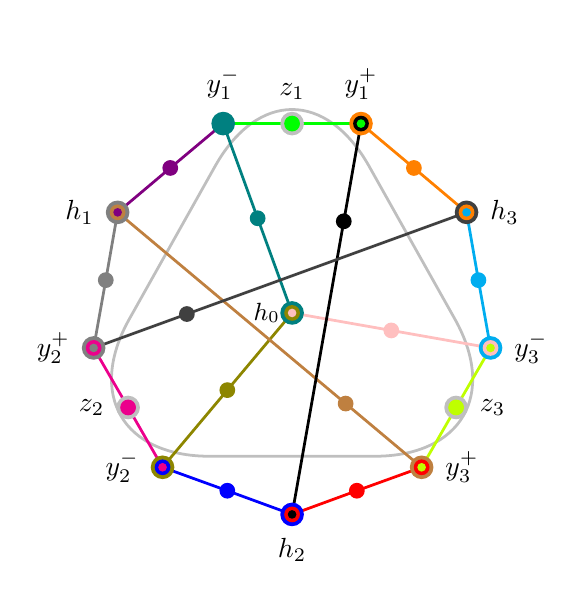
\begin{tikzpicture}  [scale=0.35]

\newdimen\ms
\ms=0.1cm

\tikzstyle{every path}=[line width=1pt]
\tikzstyle{c3}=[circle,inner sep={\ms/8},minimum size=3*\ms]
\tikzstyle{c2}=[circle,inner sep={\ms/8},minimum size=2*\ms]
\tikzstyle{c1}=[circle,inner sep={\ms/8},minimum size=1.1*\ms]



		% Define positions of all observables
		\path
     (-2.50, 6.87    ) coordinate(2)     % $y_1^-
			  (-6.33,   3.65  ) coordinate(4)    % h_1
			  (-7.20, -1.27   ) coordinate(6)       % y_2^+
			  (-4.70, -5.60   ) coordinate(8)       % y_2^-
			  (0, -7.31       ) coordinate(10)       % h_2
			  (4.70, -5.60    ) coordinate(12)        % y_3^+$
     (7.20, -1.27    ) coordinate(14)       % y_3^-
			  (6.33, 3.65     ) coordinate(16)       % h_3
			  (2.50, 6.87     ) coordinate(18)    % y_1^+

			  (0, 6.87        ) coordinate(1)     % $z_1$
			  (-4.42, 5.26    ) coordinate(3)
			  (-6.76, 1.19    ) coordinate(5)
			  (-5.95, -3.43   ) coordinate(7)     % $z_2$
			  (-2.35, -6.45   ) coordinate(9)
     (2.35, -6.45    ) coordinate(11)
			  (5.95,-3.43     ) coordinate(13)    % $z_3$
			  (6.76, 1.19     ) coordinate(15)
		   (4.42, 5.26     ) coordinate(17)

     (0,0) coordinate(19)


(0, 10.3       ) coordinate(20)     % ze1
			  (-8.7, -5.2    ) coordinate(21)     % ze2
			  (8.7,-5.2    ) coordinate(22)    % ze3


     (-1.25, 3.435 ) coordinate(23)
     (3.60, -0.635 ) coordinate(24)
     (-2.35, -2.80 ) coordinate(25)
% h1={-6.33,   3.65  }; h3p={4.70, -5.60    } ; h1d2=  (h1+h3p )/2 ; c1=  (h1d2+h3p )/2
     (1.9425, -3.2875) coordinate(26)
% h2={0, -7.31    }; h1p={2.50, 6.87   } ; h2d2=  (h2+h1p )/2 ; c2=  (h2d2+h1p )/2
     (1.875, 3.325) coordinate(27)
% h3={6.33, 3.65    }; h2p={-7.20, -1.27    } ; h3d2=  (h3+h2p )/2 ; c3=  (h3d2+h2p )/2
     (-3.8175, -0.04) coordinate(28)
;

%(4.70-6.33,   3.65  -5.60   ) coordinate(4)    % h_1

	
		% Draw all the context curves
		
\draw [rounded corners=20mm,color=lightgray]     (20) -- (21) -- (22) --  cycle;


\draw [color=green] (18) -- (1) -- (2);
\draw [color=violet] (2) -- (3) -- (4);
\draw [color=gray] (4) -- (5) -- (6);
\draw [color=magenta] (6) -- (7) -- (8);
\draw [color=blue] (8) -- (9) -- (10);
\draw [color=red] (10) -- (11) -- (12) ;

\draw [color=lime] (12) -- (13) -- (14);
\draw [color=cyan] (14) -- (15) -- (16);
\draw [color=orange] (16) -- (17) -- (18);

\draw [color=teal] (19) -- (2);
\draw [color=olive] (19) -- (8);
\draw [color=pink] (19) -- (14);

\draw [color=brown] (4) -- (12);
\draw [color=black] (10) -- (18);
\draw [color=darkgray] (16) -- (6);





%\draw [color=lightgray](0,0) circle (6.87);



\draw (19) coordinate[c3,fill=teal];
\draw (19) coordinate[c2,fill=olive];
\draw (19) coordinate[c1,fill=pink,label={[xshift=1.5pt]180:{\small $h_0$}}];


\draw (1)  coordinate[c3,fill=lightgray,label=90:$z_1$];
\draw (1)  coordinate[c2,fill=green];

\draw (2)  coordinate[c3,fill=teal,label=90:$y_1^-$];

\draw (3)  coordinate[c2,fill=violet];

\draw (4)  coordinate[c3,fill=gray,label=180:$h_1$];
\draw (4)  coordinate[c2,fill=brown];
\draw (4)  coordinate[c1,fill=violet];

\draw (5)  coordinate[c2,fill=gray,label=0:$ $];

\draw (6)  coordinate[c3,fill=darkgray,fill=gray,label=180:$y_2^+$];
\draw (6)  coordinate[c2,fill=magenta];
\draw (6)  coordinate[c1,fill=gray];

\draw (7)  coordinate[c3,fill=lightgray,label=180:$z_2$];
\draw (7)  coordinate[c2,fill=magenta];

\draw (8)  coordinate[c3,fill=olive,label=180:$y_2^-$];
\draw (8)  coordinate[c2,fill=blue];
\draw (8)  coordinate[c1,fill=magenta];

\draw (9)  coordinate[c2,fill=blue,label=0:$ $];

\draw (10) coordinate[c3,fill=blue,label=270:$h_2$];
\draw (10) coordinate[c2,fill=red];
\draw (10) coordinate[c1,fill=black];

\draw (11) coordinate[c2,fill=red,label=0:$ $];

\draw (12) coordinate[c3,fill=brown,label=0:$y_3^+$];
\draw (12) coordinate[c2,fill=red];
\draw (12) coordinate[c1,fill=lime];

\draw (13) coordinate[c3,fill=lightgray,label=0:$z_3$];
\draw (13) coordinate[c2,fill=lime];

\draw (14) coordinate[c3,fill=cyan,label=0:$y_3^-$];
\draw (14) coordinate[c2,fill=pink];
\draw (14) coordinate[c1,fill=lime];

\draw (15) coordinate[c2,fill=cyan,label=0:$ $];

\draw (16) coordinate[c3,fill=darkgray,label=0:$h_3$];
\draw (16) coordinate[c2,fill=orange];
\draw (16) coordinate[c1,fill=cyan];

\draw (17) coordinate[c2,fill=orange,label=0:$ $];

\draw (18) coordinate[c3,fill=orange,label=90:$y_1^+$];
\draw (18) coordinate[c2,fill=black];
\draw (18) coordinate[c1,fill=green];

\draw (23) coordinate[c2,fill=teal];
\draw (24) coordinate[c2,fill=pink];
\draw (25) coordinate[c2,fill=olive];
\draw (26) coordinate[c2,fill=brown];
\draw (27) coordinate[c2,fill=black];
\draw (28) coordinate[c2,fill=darkgray];


		\end{tikzpicture}
&
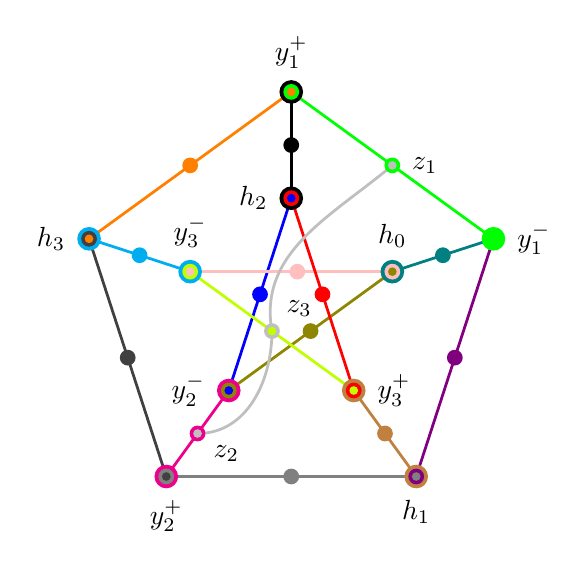
\begin{tikzpicture}  [scale=0.45]
\newdimen\ms
\ms=0.1cm

\tikzstyle{every path}=[line width=1pt]
\tikzstyle{c3}=[circle,inner sep={\ms/8},minimum size=3*\ms]
\tikzstyle{c2}=[circle,inner sep={\ms/8},minimum size=2*\ms]
\tikzstyle{c1}=[circle,inner sep={\ms/8},minimum size=1.1*\ms]

% Radius of regular polygons
\newdimen\R
\R=6cm
%\r= { \R * sqrt(3)/2}
\newdimen\K
\K=3cm

% Define positions of all observables
\path
  ({90 + 0 * 360 /5}:\R      ) coordinate(1)
  ({90 + 360 /10 + 0 * 360/5} : {\R * 0.6881/0.8507} ) coordinate(2)
  ({90 + 1 * 360 /5}:\R   ) coordinate(3)
  ({90 + 360 /10 + 1 * 360/5} : {\R * 0.6881/0.8507} ) coordinate(4)
  ({90 + 2 * 360 /5}:\R  ) coordinate(5)
  ({90 + 360 /10 + 2 * 360/5} : {\R * 0.6881/0.8507} ) coordinate(6)
  ({90 + 3 * 360 /5}:\R  ) coordinate(7)
  ({90 + 360 /10 + 3 * 360/5} : {\R * 0.6881/0.8507} ) coordinate(8)
  ({90 + 4 * 360 /5}:\R     ) coordinate(9)
  ({90 + 360 /10 + 4 * 360/5} : {\R * 0.6881/0.8507} ) coordinate(10)
  ({90 + 0 * 360 /5}:\K      ) coordinate(11)
  ({90 + 360 /10 + 0 * 360/5} : {\K * 0.6881/0.8507} ) coordinate(12)
  ({90 + 1 * 360 /5}:\K   ) coordinate(13)
  ({90 + 360 /10 + 1 * 360/5} : {\K * 0.6881/0.8507} ) coordinate(14)
  ({90 + 2 * 360 /5}:\K  ) coordinate(15)
  ({90 + 360 /10 + 2 * 360/5} : {\K * 0.6881/0.8507} ) coordinate(16)
  ({90 + 3 * 360 /5}:\K  ) coordinate(17)
  ({90 + 360 /10 + 3 * 360/5} : {\R * 0.6881/0.8507} ) coordinate(18)
  ({90 + 4 * 360 /5}:\K     ) coordinate(19)
  ({90 + 360 /10 + 4 * 360/5} : {\K * 0.6881/0.8507} ) coordinate(20)

  ({90 + 2 * 360 /5}:{(\R+\K)/2}) coordinate(21)

;

% draw contexts

\draw [color=orange] (1) -- (2) -- (3);
\draw [color=darkgray] (3) -- (4) -- (5);
\draw [color=gray] (5) -- (6) -- (7);
\draw [color=violet] (7) -- (8) -- (9);
\draw [color=green] (9) -- (10) -- (1);    %

\draw [color=blue] (11) -- (15) ;
\draw [color=olive] (15) -- (19);
\draw [color=pink] (19) -- (13);
\draw [color=lime] (13) -- (17);
\draw [color=red] (17) -- (11);

\draw ($ (11) !.5! (15) $) coordinate[c2,fill=blue];  %
\draw ($ (15) !.5! (19) $) coordinate[c2,fill=olive];  %
\draw ($ (19) !.47! (13) $) coordinate[c2,fill=pink];  %
\draw ($ (17) !.5! (11) $) coordinate[c2,fill=red];  %

\draw [color=black] (1) -- (11);
\draw [color=cyan] (3) -- (13);
\draw [color=magenta] (5) -- (15);
\draw [color=brown] (7) -- (17);
\draw [color=teal] (9) -- (19);

\draw ($ (1) !.5! (11) $) coordinate[c2,fill=black];  %
\draw ($ (3) !.5! (13) $) coordinate[c2,fill=cyan];  %
\draw ($ (7) !.5! (17) $) coordinate[c2,fill=brown];  %
\draw ($ (9) !.5! (19) $) coordinate[c2,fill=teal];  %

\draw [color=lightgray] (10)  to   [out=-140,in=100] ($ (13) !.5! (17) $)  to   [out=-90,in=0] (21);
%
%%
%% draw atoms
%%
%
\draw (1) coordinate[c3,fill=black,label=90:$y_1^+$];  %
\draw (1) coordinate[c2,fill=green];   %
\draw (1) coordinate[c1,fill=orange];  %
%
\draw (2) coordinate[c2,fill=orange];    %
%
\draw (3) coordinate[c3,fill=cyan,label=180:$h_3$];   %
\draw (3) coordinate[c2,fill=darkgray]; %
\draw (3) coordinate[c1,fill=orange];  %
%
\draw (4) coordinate[c2,fill=darkgray];  %
%
\draw (5) coordinate[c3,fill=magenta,label=270:$y_2^+$];  %
\draw (5) coordinate[c2,fill=gray];  %
\draw (5) coordinate[c1,fill=darkgray];  %
%
\draw (6) coordinate[c2,fill=gray];
%
\draw (7) coordinate[c3,fill=brown,label=270:$h_1$];  %
\draw (7) coordinate[c2,fill=violet];  %
\draw (7) coordinate[c1,fill=gray];  %
%
\draw (8) coordinate[c2,fill=violet];  %
%
\draw (9) coordinate[c3,fill=green,label=0:$y_1^-$];
%
\draw (10) coordinate[c2,fill=green,label=0:$z_1$];  %
\draw (10) coordinate[c1,fill=lightgray];  %
%
\draw (11) coordinate[c3,fill=black,label=180:$h_2$];  %
\draw (11) coordinate[c2,fill=red];  %
\draw (11) coordinate[c1,fill=blue]; %
%
%
\draw (13) coordinate[c3,fill=cyan,label=90:$y_3^-$]; %
\draw (13) coordinate[c2,fill=lime];  %
\draw (13) coordinate[c1,fill=pink];  %
%
\draw (15) coordinate[c3,fill=magenta,label=180:$y_2^-$]; %
\draw (15) coordinate[c2,fill=olive]; %
\draw (15) coordinate[c1,fill=blue]; %

\draw (17) coordinate[c3,fill=brown,label=0:$y_3^+$];  %
\draw (17) coordinate[c2,fill=red];   %
\draw (17) coordinate[c1,fill=lime]; %

\draw (19) coordinate[c3,fill=teal,label=90:$h_0$]; %
\draw (19) coordinate[c2,fill=pink]; %
\draw (19) coordinate[c1,fill=olive]; %

%
\draw (21) coordinate[c2,fill=magenta];  %
\draw (21) coordinate[c1,fill=lightgray,label=-15:$z_2$];  %

\draw ($ (13) !.5! (17) $) coordinate[c2,fill=lightgray];  %
\draw ($ (13) !.5! (17) $) coordinate[c1,fill=lime,label=45:$z_3$];  %


\end{tikzpicture}
\end{tabular}
}
\end{center}

\end{frame}


\begin{frame}{Set Representable Chromatic Kochen-Specker Contextuality}
Hypergraph representations of $G_{32}$ (Greechie, 1971, Figure~6,
\href{https://doi.org/10.1016/0097-3165(71)90015-X}{doi:10.1016/0097-3165(71)90015-X})
which is set representable (with a separating set of two-valued states) as partition logic, as depicted.
It has \alert{clique number 3} (3 elements per hyperedge/block), yet \alert{chromatic number $\chi(G_{32} = 4$}.
\alert{All 6 two-valued states are non-aggregated!}

Proof in Shekarriz and KS (2022, \href{https://doi.org/10.1063/5.0062801}{doi:10.1063/5.0062801}).
% It's good practice to define colors if you use them, especially non-standard ones.
% For portability, we'll stick to the mixed color from the first figure.


\begin{center}
    \begin{tabular}{ c c c }
        \resizebox{0.4\textwidth}{!}{%
            % --- FIGURE 1 (Original) ---
            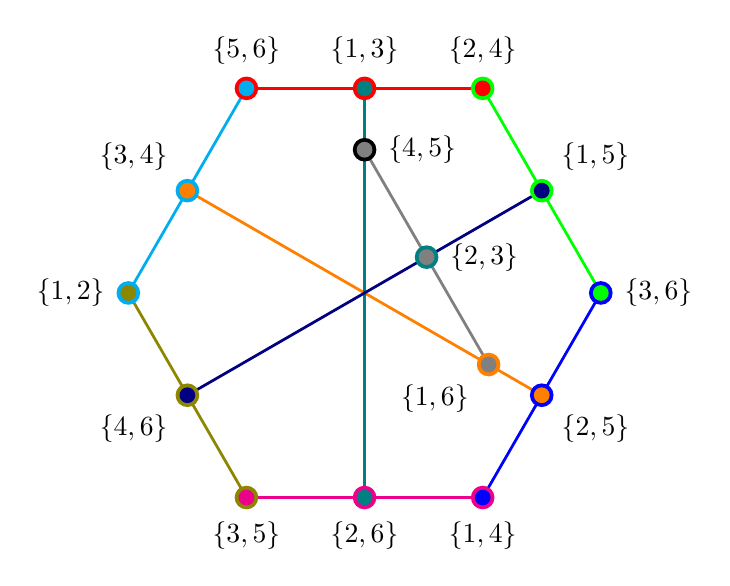
\begin{tikzpicture}

                \tikzset{
                    every path/.style={line width=1pt},
                    c3/.style={circle, inner sep={0.05cm/8}, minimum size=6*0.05cm},
                    c2/.style={circle, inner sep={0.05cm/8}, minimum size=4*0.05cm},
                    c1/.style={circle, inner sep={0.05cm/8}, minimum size=0.8*0.05cm}
                }

                \def\R{30mm}

                % Define positions of all observables
                \path
                ({ 180 - 0 * 360 /6}:\R)      coordinate(1)
                ({ 180 - 30 - 0 * 360 /6}:{\R * sqrt(3)/2})      coordinate(2)
                ({ 180 - 1 * 360 /6}:\R)   coordinate(3)
                ({ 180 - 30 - 1 * 360 /6}:{\R * sqrt(3)/2})   coordinate(4)
                ({ 180 - 2 * 360 /6}:\R)  coordinate(5)
                ({ 180 - 30 - 2 * 360 /6}:{\R * sqrt(3)/2})  coordinate(6)
                ({ 180 - 3 * 360 /6}:\R)  coordinate(7)
                ({ 180 - 30 - 3 * 360 /6}:{\R * sqrt(3)/2})  coordinate(8)
                ({ 180 - 4 * 360 /6}:\R)     coordinate(9)
                ({ 180 - 30 - 4 * 360 /6}:{\R * sqrt(3)/2})     coordinate(10)
                ({ 180 - 5 * 360 /6}:\R)     coordinate(11)
                ({ 180 - 30 - 5 * 360 /6}:{\R * sqrt(3)/2})     coordinate(12)
                ;

                % Draw contexts (lines)
                \draw [color=cyan] (1) -- (2) -- (3);
                \draw [color=red] (3) -- (4) -- (5);
                \draw [color=green] (5) -- (6) -- (7);
                \draw [color=blue] (7) -- (8) -- (9);
                \draw [color=magenta] (9) -- (10) -- (11);
                \draw [color=olive] (11) -- (12) -- (1);
                \draw [color=orange] (2) -- (8)  coordinate[pos=0.85]  (15);
                \draw [color=teal] (4) -- (10)  coordinate[pos=0.15]  (13);
                \draw [color=blue!50!black] (6) -- (12)  coordinate[pos=0.325]  (14);
                \draw [color=gray] (13) --(15);

                % Draw atoms (nodes)
                \draw (1) coordinate[c3,fill=cyan,label={left: $\{ 1,2\} $}];
                \draw (1) coordinate[c2,fill=olive];
                \draw (2) coordinate[c3,fill=cyan,label={above left: $\{ 3,4\}$}];
                \draw (2) coordinate[c2,fill=orange];
                \draw (3) coordinate[c3,fill=red,label={above: $\{ 5,6\} $}];
                \draw (3) coordinate[c2,fill=cyan];
                \draw (4) coordinate[c3,fill=red,label={above: $\{ 1,3\}$}];
                \draw (4) coordinate[c2,fill=teal];
                \draw (5) coordinate[c3,fill=green,label={above: $\{ 2,4\} $}];
                \draw (5) coordinate[c2,fill=red];
                \draw (6) coordinate[c3,fill=green,label={above right: $\{ 1,5\} $}];
                \draw (6) coordinate[c2,fill=blue!50!black];
                \draw (7) coordinate[c3,fill=blue,label={right: $\{ 3,6\}$}];
                \draw (7) coordinate[c2,fill=green];
                \draw (8) coordinate[c3,fill=blue,label={below right: $\{ 2,5\}$}];
                \draw (8) coordinate[c2,fill=orange];
                \draw (9) coordinate[c3,fill=magenta,label={below: $\{ 1,4\}$}];
                \draw (9) coordinate[c2,fill=blue];
                \draw (10) coordinate[c3,fill=magenta,label={below: $\{ 2,6\}$}];
                \draw (10) coordinate[c2,fill=teal];
                \draw (11) coordinate[c3,fill=olive,label={below: $\{ 3,5\}$}];
                \draw (11) coordinate[c2,fill=magenta];
                \draw (12) coordinate[c3,fill=olive,label={below left: $\{ 4,6\}$}];
                \draw (12) coordinate[c2,fill=blue!50!black];
                \draw (13) coordinate[c3,fill,label={right: $\{ 4,5\}$}];
                \draw (13) coordinate[c2,fill=gray];
                \draw (14) coordinate[c3,fill=teal,label=0:{$\{ 2,3\}$}];
                \draw (14) coordinate[c2,fill=gray];
                \draw (15) coordinate[c3,fill=orange,label={below left: $\{1,6\}$}];
                \draw (15) coordinate[c2,fill=gray];

            \end{tikzpicture}
        } % end of resizebox
        & \qquad &
        \resizebox{0.4\textwidth}{!}{%
            % --- FIGURE 2 (Color-substituted: blue -> orange) ---
            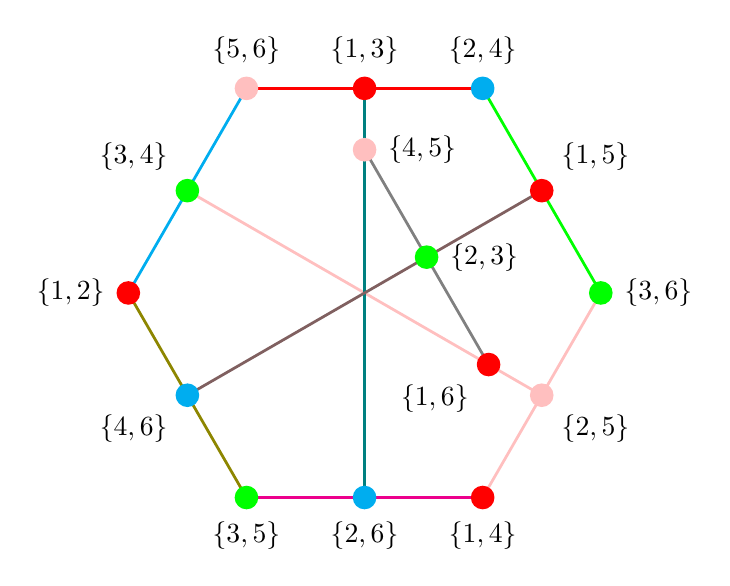
\begin{tikzpicture}

                \tikzset{
                    every path/.style={line width=1pt},
                    c3/.style={circle, inner sep={0.05cm/8}, minimum size=6*0.05cm},
                    c2/.style={circle, inner sep={0.05cm/8}, minimum size=4*0.05cm},
                    c1/.style={circle, inner sep={0.05cm/8}, minimum size=0.8*0.05cm}
                }

                \def\R{30mm}

                % Define positions of all observables
                \path
                ({ 180 - 0 * 360 /6}:\R)      coordinate(1)
                ({ 180 - 30 - 0 * 360 /6}:{\R * sqrt(3)/2})      coordinate(2)
                ({ 180 - 1 * 360 /6}:\R)   coordinate(3)
                ({ 180 - 30 - 1 * 360 /6}:{\R * sqrt(3)/2})   coordinate(4)
                ({ 180 - 2 * 360 /6}:\R)  coordinate(5)
                ({ 180 - 30 - 2 * 360 /6}:{\R * sqrt(3)/2})  coordinate(6)
                ({ 180 - 3 * 360 /6}:\R)  coordinate(7)
                ({ 180 - 30 - 3 * 360 /6}:{\R * sqrt(3)/2})  coordinate(8)
                ({ 180 - 4 * 360 /6}:\R)     coordinate(9)
                ({ 180 - 30 - 4 * 360 /6}:{\R * sqrt(3)/2})     coordinate(10)
                ({ 180 - 5 * 360 /6}:\R)     coordinate(11)
                ({ 180 - 30 - 5 * 360 /6}:{\R * sqrt(3)/2})     coordinate(12)
                ;

                % Draw contexts (lines) with colors substituted
                \draw [color=cyan] (1) -- (2) -- (3);
                \draw [color=red] (3) -- (4) -- (5);
                \draw [color=green] (5) -- (6) -- (7);
                \draw [color=pink] (7) -- (8) -- (9); % Changed from blue
                \draw [color=magenta] (9) -- (10) -- (11);
                \draw [color=olive] (11) -- (12) -- (1);
                \draw [color=pink] (2) -- (8)  coordinate[pos=0.85]  (15);
                \draw [color=teal] (4) -- (10)  coordinate[pos=0.15]  (13);
                \draw [color=pink!50!black] (6) -- (12)  coordinate[pos=0.325]  (14); % Changed from blue!50!black
                \draw [color=gray] (13) --(15);

                % Draw atoms (nodes) with colors substituted
                \draw (1) coordinate[c3,fill=red,label={left: $\{ 1,2\} $}];
                \draw (2) coordinate[c3,fill=green,label={above left: $\{ 3,4\}$}];
                \draw (3) coordinate[c3,fill=pink,label={above: $\{ 5,6\} $}]; % Changed from blue
                \draw (4) coordinate[c3,fill=red,label={above: $\{ 1,3\}$}];
                \draw (5) coordinate[c3,fill=cyan,label={above: $\{ 2,4\} $}];
                \draw (6) coordinate[c3,fill=red,label={above right: $\{ 1,5\} $}];
                \draw (7) coordinate[c3,fill=green,label={right: $\{ 3,6\}$}];
                \draw (8) coordinate[c3,fill=pink,label={below right: $\{ 2,5\}$}]; % Changed from blue
                \draw (9) coordinate[c3,fill=red,label={below: $\{ 1,4\}$}];
                \draw (10) coordinate[c3,fill=cyan,label={below: $\{ 2,6\}$}];
                \draw (11) coordinate[c3,fill=green,label={below: $\{ 3,5\}$}];
                \draw (12) coordinate[c3,fill=cyan,label={below left: $\{ 4,6\}$}];
                \draw (13) coordinate[c3,fill=pink,label={right: $\{ 4,5\}$}]; % Changed from blue
                \draw (14) coordinate[c3,fill=green,label=0:{$\{ 2,3\}$}];
                \draw (15) coordinate[c3,fill=red,label={below left: $\{1,6\}$}];

            \end{tikzpicture}
        } % end of resizebox
    \end{tabular}
\end{center}


\end{frame}

%\begin{frame}{Spectral Decomposition: Maximal vs. Degenerate, ``full operator-valued versus two-valued'' }
%    Let $\{\ket{\mathbf{e}_i} \mid 1 \le i \le d\}$ be an orthonormal basis.
%    \begin{block}{Maximal Operator (von Neumann, 1931)}
%    Outcomes $\lambda_i$ are mutually distinct (unique "colors"):
%    \[ A = \sum_{i=1}^d \lambda_i \ket{\mathbf{e}_i}\bra{\mathbf{e}_i} \]
%    \end{block}
%    \pause
%    \begin{block}{Degenerate Operator (Projector)}
%    Only two outcomes (e.g., 1 for state $j$, 0 otherwise):
%    \[ P_j = \ket{\mathbf{e}_j}\bra{\mathbf{e}_j} = \sum_{i=1}^d \delta_{ij} \ket{\mathbf{e}_i}\bra{\mathbf{e}_i} \]
%    \end{block}
%\end{frame}



\begin{frame}{Results on Chromatic Contextuality}

{Colorings---unlike two-valued states---represent the maximal information that is empirical available, as they fix the measurement context.
They thus represent a formidable tool to identify and investigate quantum contextuality
(as per differences in classical-versus-quantum predictions):}

    \begin{itemize}[<+->] % Reveals items one by one
        \item \alert{Chromatic Kochen-Specker Theorem:} There exist finite set as well as FOR (Hilbert space) representable collections of observables
where the chromatic number of the associated $d$-uniform hypergraph $G$ exceeds the
 clique number or associated Hilbert space dimension, that is, $\chi(G) > d$.

        \item \alert{Non-Aggregated Two-Valued States:} There exist  two-valued states   on $d$-uniform hypergraphs
       that either cannot be generated by aggregating any of its $d$-colorings,
       or are present even in the absence of any coloring.


    \end{itemize}
\end{frame}

\frame{

\centerline{\Large {\color{magenta} Thank you for your attention!}}

\begin{center}\color{pink}
$\widetilde{\qquad \qquad }$
$\widetilde{\qquad \qquad}$
$\widetilde{\qquad \qquad }$
\end{center}
 }

\end{document}

%==================================================================
\section{Understanding Information}
%==================================================================
\begin{frame}{Shannon Entropy: Quantifying Information}
    \begin{itemize}
        \item Shannon Entropy ($H$) measures the \alert{average uncertainty} or \alert{information content} of a random variable.
        \item The more uncertain an outcome, the higher its entropy, and the more information we gain upon observation.
        \item It's typically measured in \alert{bits} (when using $\log_2$).
    \end{itemize}
    \pause
    \begin{block}{Formula for Shannon Entropy}
        For a discrete random variable $X$ with outcomes $x_i$ and probabilities $P(x_i)$:
        \begin{equation*}
            H(X) = -\sum_{i=1}^{n} P(x_i) \log_2 P(x_i)
        \end{equation*}
    \end{block}
    \pause
    \begin{alertblock}{Core Assumption}
        For the following examples, we assume the initial underlying states are \textbf{equiprobable}.
    \end{alertblock}
\end{frame}

%==================================================================
\section{3-State System Analysis}
%==================================================================
\begin{frame}{3-State System: Full Resolution}
    \begin{itemize}
        \item \textbf{System:} 3 distinct, equiprobable states.
        \item \textbf{Observed Outcomes:} $\{0, 1, 2\}$
        \item \textbf{Probabilities:} $P(0) = P(1) = P(2) = 1/3$
    \end{itemize}
    \pause
    \begin{block}{Calculating Information ($\Hfull$)}
        \begin{align*}
            \Hfull &= - \sum_{i=0}^{2} \frac{1}{3} \log_2 \left(\frac{1}{3}\right) \\
            &= -3 \times \frac{1}{3} \log_2 \left(\frac{1}{3}\right) = \log_2(3) \\
            &\approx \SI{1.585}{bits}
        \end{align*}
    \end{block}
\end{frame}

\begin{frame}{3-State System: Aggregated Resolution}
    \begin{itemize}
        \item \textbf{Mapping (Aggregation):}
             $0 \to \obs{0}$, \quad $1 \to \obs{1}$, \quad $2 \to \obs{1}$
        \item \textbf{New Observed Outcomes:} $\{\obs{0}, \obs{1}\}$
        \item \textbf{New Probabilities:}
            \begin{align*}
                P(\obs{0}) &= P(0) = 1/3 \\
                P(\obs{1}) &= P(1) + P(2) = 2/3
            \end{align*}
    \end{itemize}
    \pause
    \begin{block}{Calculating Information ($\Hcoll$)}
        \begin{align*}
            \Hcoll &= - \left[ \frac{1}{3} \log_2 \left(\frac{1}{3}\right) + \frac{2}{3} \log_2 \left(\frac{2}{3}\right) \right] \\
            &\approx \SI{0.918}{bits}
        \end{align*}
    \end{block}
\end{frame}

\begin{frame}{3-State System: Summary}
    \begin{columns}[T] % Aligns the top of the columns
        \begin{column}{0.5\textwidth}
            \begin{itemize}
                \item \textbf{Full Resolution:} \\ $\Hfull \approx \alert{\SI{1.585}{bits}}$
                \vspace{1em}
                \item \textbf{Aggregated Resolution:} \\ $\Hcoll \approx \alert{\SI{0.918}{bits}}$
            \end{itemize}
        \end{column}
        \begin{column}{0.5\textwidth}
            \pause
            \begin{block}{Information Loss}
                The aggregation reduces the information obtained.
                \begin{align*}
                    \text{Loss} &= \Hfull - \Hcoll \\
                    &\approx 1.585 - 0.918 \\
                    &= \mathbf{\SI{0.667}{bits}}
                \end{align*}
            \end{block}
        \end{column}
    \end{columns}
\end{frame}

%==================================================================
\section{4-State System Analysis}
%==================================================================
\begin{frame}{4-State System: Full Resolution}
    \begin{itemize}
        \item \textbf{System:} 4 distinct, equiprobable states.
        \item \textbf{Observed Outcomes:} $\{0, 1, 2, 3\}$
        \item \textbf{Probabilities:} $P(0) = P(1) = P(2) = P(3) = 1/4$
    \end{itemize}
    \pause
    \begin{block}{Calculating Information ($\Hfull$)}
        \begin{align*}
            \Hfull &= - \sum_{i=0}^{3} \frac{1}{4} \log_2 \left(\frac{1}{4}\right) = \log_2(4) \\
            &= \SI{2}{bits}
        \end{align*}
        \alert{A 4-state equiprobable system perfectly encodes 2 bits.}
    \end{block}
\end{frame}

\begin{frame}{4-State System: Aggregated Cases}
    \begin{columns}[T]
        \begin{column}{0.5\textwidth}
            \begin{block}{Case A: Symmetric Aggregation}
                $\{0, 1\} \to \obs{0}$ \\
                $\{2, 3\} \to \obs{1}$
                \pause
                \begin{align*}
                    P(\obs{0}) &= 1/2 \\
                    P(\obs{1}) &= 1/2 \\
                    \HcaseA &= \SI{1}{bit}
                \end{align*}
                \alert<3>{Like a fair coin flip.}
            \end{block}
        \end{column}
        \begin{column}{0.5\textwidth}
            \pause
            \begin{block}{Case B: Asymmetric Aggregation}
                $\{0, 1, 2\} \to \obs{0}$ \\
                $\{3\} \to \obs{1}$
                \pause
                \begin{align*}
                    P(\obs{0}) &= 3/4 \\
                    P(\obs{1}) &= 1/4 \\
                    \HcaseB &\approx \SI{0.811}{bits}
                \end{align*}
            \end{block}
        \end{column}
    \end{columns}
\end{frame}


\begin{frame}{4-State System: Summary}
    \begin{itemize}
        \item \textbf{Full Resolution:} $\Hfull = \alert{\SI{2}{bits}}$
        \item \textbf{Case A (Symmetric):} $\HcaseA = \alert{\SI{1}{bit}}$
        \item \textbf{Case B (Asymmetric):} $\HcaseB \approx \alert{\SI{0.811}{bits}}$
    \end{itemize}
    \pause
    \begin{block}{Observation}
        Each state aggregation leads to a \alert{reduction} in measurable information. The more states are merged and the more skewed the resulting probabilities, the lower the entropy.
    \end{block}
\end{frame}

